\documentclass[12pt,a4paper]{article}

% --- Balíčky pro češtinu a kódování ---
\usepackage[utf8]{inputenc}
\usepackage[english, czech]{babel}
\usepackage[T1]{fontenc}
\usepackage{parskip}

\usepackage[margin=2.5cm]{geometry}

\usepackage[pdftex]{graphicx}
\usepackage{listings} % Pro vkládání zdrojového kódu
\usepackage{xcolor}   % Pro barvy v kódu
\usepackage{hyperref} % Odkazy v PDF
\usepackage{amsmath}  % Matematika (matice)
\usepackage{graphicx}
\usepackage{wrapfig}
\usepackage{float}

\usepackage{url}


\title{Rainfall Engine: Architektura a implementace herního enginu v C++}
\author{Adam Švec}
\date{\today}


% --- Nastavení vzhledu kódu (C++) ---
\definecolor{codegreen}{rgb}{0,0.6,0}
\definecolor{codegray}{rgb}{0.5,0.5,0.5}
\definecolor{codepurple}{rgb}{0.58,0,0.82}
\definecolor{backcolour}{rgb}{0.95,0.95,0.95}

\lstset{
    language=C++,
    backgroundcolor=\color{backcolour},
    commentstyle=\color{codegreen},
    keywordstyle=\color{blue},
    numberstyle=\tiny\color{codegray},
    stringstyle=\color{codepurple},
    basicstyle=\ttfamily\small,
    breaklines=true,
    numbers=left,
    showstringspaces=false
}


% Titulní strana
\begin{document}

\begin{titlepage}
    \centering

    
\includegraphics[width=6cm]{SPSE-Jecna_Logo.pdf}

    \vspace*{0.25cm}
    {\huge\bfseries Střední průmyslová škola elektrotechnická, Ječná 30, 12 000, Praha 2 \par}

    \vspace{2cm}
    {\Large Odborná práce \par}

    \vspace{2cm}
    {\huge\bfseries Rainfall Engine: Architektura a implementace herního enginu v C++ \par}

    \vspace{1.5cm}
    {\Large \textbf{Adam Švec} \par}

    \vfill
    {\Large \today \par}
\end{titlepage}


% Anotace
\pagenumbering{roman}
\renewenvironment{abstract}{
  \small
  \begin{center}
    \bfseries \abstractname\vspace{-.5em}\vspace{0pt}
  \end{center}
  \quotation
}{\endquotation}

\begin{abstract}
    Tato práce se zabývá návrhem a realizací herního enginu zaměřeného na 3D počítačovou grafiku. Hlavním cílem projektu bylo vytvořit softwarovou knihovnu v jazyce C++ pro vývoj her a doprovodný editor pro platformu Windows, který umožňuje vizuální úpravy scén v reálném čase. Jádro systému využívá grafické rozhraní OpenGL pro efektivní vykreslování na obrazovku a jazyk GLSL pro programování shaderů. Pro správu herních objektů a jejich dat byl implementován moderní návrhový vzor Entity Component System (ECS), který zajišťuje vysokou flexibilitu a výkon. Výsledkem je plně funkční knihovna a editor, jejichž možnosti jsou demonstrovány na přiložené ukázkové hře. Vytvořené řešení poskytuje přehledné prostředí pro snadné vytváření 3D aplikací a slouží jako praktická ukázka implementace nízkoúrovňových grafických technologií.
\end{abstract}
\noindent \textbf{Klíčová slova:} OpenGL, C++, herní engine, počítačová grafika, vývoj her

\vspace{1.5cm}

\selectlanguage{english}

\begin{abstract}
    This thesis focuses on the design and implementation of a game engine centered on 3D computer graphics. The primary objective of the project was to develop a C++ software library for game development alongside a dedicated Windows-based editor that enables real-time visual scene manipulation. The core system utilizes the OpenGL graphics API for efficient rendering and GLSL for shader programming. To manage game objects and data, a modern Entity Component System (ECS) design pattern was implemented, ensuring high flexibility and performance. The final result is a fully functional library and editor, the capabilities of which are demonstrated through a provided sample game. This solution offers a streamlined environment for 3D application development and serves as a practical demonstration of low-level graphics technology implementation.
\end{abstract}
\noindent \textbf{Keywords:} OpenGL, C++, Game Engine, Computer Graphics, Game Development

\selectlanguage{czech}
\newpage



% Obsah
\setcounter{tocdepth}{3}
\tableofcontents
\newpage



\pagenumbering{arabic}
\section{Úvod}
Hlavní motivací pro vznik této práce a samotného projektu Rainfall Engine byla touha do hloubky pochopit, jak herní enginy reálně fungují, jak spravují paměť a jakým způsobem komunikují s grafickou kartou. Celý projekt původně odstartoval pouze jako osobní experiment a koníček pramenící z mé vášně pro počítačovou grafiku a vizuální tvorbu.

Mým dlouhodobým profesním cílem je působit v herním průmyslu na pozici vývojáře enginů (\textit{Engine Developer}) s úzkou specializací na počítačovou grafiku. Vytvoření vlastního enginu od úplných základů v jazyce C++ tak představuje nezbytný a logický krok k dosažení tohoto cíle. Nejedná se o pokus vytvořit konkurenci zavedeným komerčním řešením, ale spíše o funkční demonstraci schopnosti navrhnout a naimplementovat vlastní škálovatelnou architekturu.

Při vývoji enginu a sepisování této dokumentace bylo čerpáno z odborných zdrojů a dokumentace k využitým knihovnám, které jsou detailně uvedeny v seznamu literatury na konci práce.


\section{Použité technologie}

\subsection{C++}
Pro naprogramování herního enginu je vhodný jazyk \texttt{C++}, díky jeho rychlosti a nízkoúrovňovému přístupu k paměti. Všechny grafické knihovny jako jsou OpenGL a DirectX jsou primárně vyvíjeny pro C++, tudíž nemusím používat verze třetích stran.

Většina veřejných a proprietárních enginů je primárně vytvářeno v C++, a protože bych jednou chtěl pracovat pro herní studio jako engine vývojář, zkušenost pracovat v C++ s herním enginem bude velmi užitečná.

\subsection{OpenGL}
\texttt{OpenGL} je grafické API (\textit{Application Programming Interface}), které nám umožňuje vykreslovat trojúhelníky na obrazovku. K vykreslování využívá grafickou kartu (\textit{GPU}), která byla pro tuto práci specificky stvořena, tudíž je několikanásobně rychlejší, než kdybychom vykreslovali přes procesor (\textit{CPU}).

Abychom se mohli dostat k funkcím \texttt{OpenGL}, musíme použít knihovnu, jako je \texttt{GLAD}, která nám je poskytne.

\subsection{GLFW}
\texttt{GLFW} dovoluje vytvořit okno, do kterého lze následně cokoliv vykreslovat, pomocí OpenGL. Také umožňuje zachycovat uživatelský vstup, jako je klávesnice a myš. \texttt{GLFW} je knihovna, která je specificky mířena na \texttt{OpenGL}, tudíž vhodnou volbou.

\subsection{CMake}
\texttt{CMake} vytváří adresářovou strukturu a kompiluje za nás kód do knihoven a spustitelných souborů (\textit{.exe}).

\subsection{Uživatelské prostředí} \label{sec:tech-ui}
Herní uživatelské prostředí (\textit{User Interface}) může uživatel enginu vytvářet pomocí knihovny \texttt{RmlUi}. RmlUi funguje na bázi HTML a CSS, což poskytuje povědomé prostředí pro většinu uživatelů a umožňuje velkou kreativitu ve vzhledu uživatelského prostředí.

Editor používá na uživatelské prostředí knihovnu \texttt{Dear ImGui}, kvůli její jednoduchosti a rychlé iteraci a úpravy jednotlivách elementů.

\subsection{Načítání a ukládání}
K načítání textur používá engine jednoheaderovou knihovnu \texttt{stb\_image.h}, která bohatě stačí k načítáná většiny populárních formátů. Podobně k načítání 3D modélů engine používá knihovnu Assimp, která podporuje řadu formátů. Tyto knihovny jsem vybral, díky jejich jednoduchosti a jejich přístupným návodům.

Na ukládání a načítání scén a projektů do souborů jsem vybral formát YAML, který používá i Unity na ukládaní svých scén. Pro tento úkol používá engine knihovnu \texttt{yaml-cpp}.



\section{Struktura enginu}
Celý engine váže třída \texttt{engine::Engine}, která vše vlastní a spouští. Inicializují se v ní všechny hlavní komponenty spolu s hlavní herní smyčkou (\textit{game loop}).

\begin{figure}[H]
    \centering
    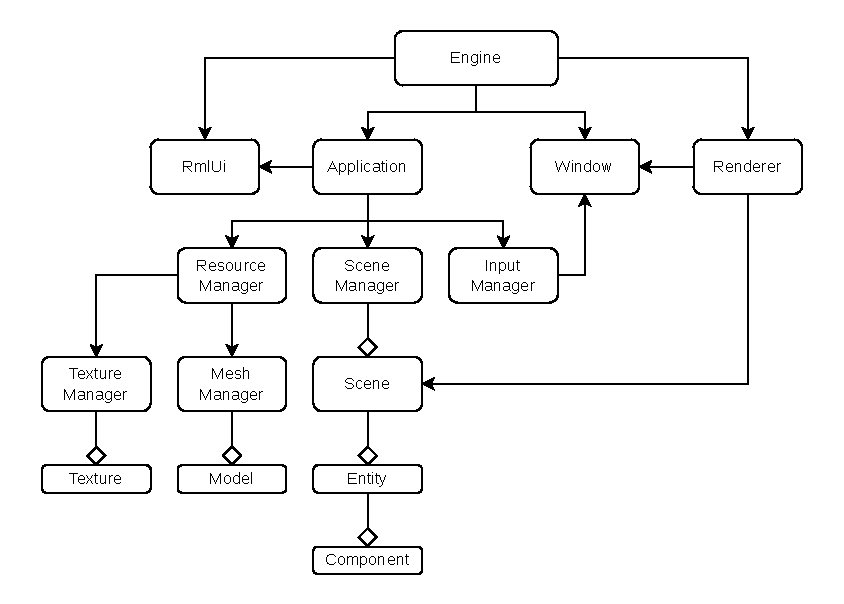
\includegraphics[width=0.8\textwidth]{engine_diagram.pdf}
    \caption{Diagram architektury enginu}
    \label{fig:architektura}
\end{figure}


\subsection{Window}
Pomocí knihovny GLFW zajišťuje vytvoření okna a zachycuje uživatelský vstup, který následně používá Input Manager a RmlUi.


\subsection{Renderování}
Renderer vykresluje aktuální scénu pomocí OpenGL.

\subsubsection{Shadery a vykreslovací řetězec}
\texttt{Shadery} pro OpenGL jsou psány v GLSL (\textit{OpenGL Shading Language}), který je založen na syntaxi jazyku \texttt{C}. Je to způsob jak psát kód na grafické kartě. Existuje spousta různých typů shaderů a každý je vhodný na něco jiného. Dva nejdůležitější shadery jsou \textit{vertex} a \textit{fragment} shadery, bez kterých nemůžeme nic vykreslovat na obrazovku.

\begin{figure}[H]
    \centering
    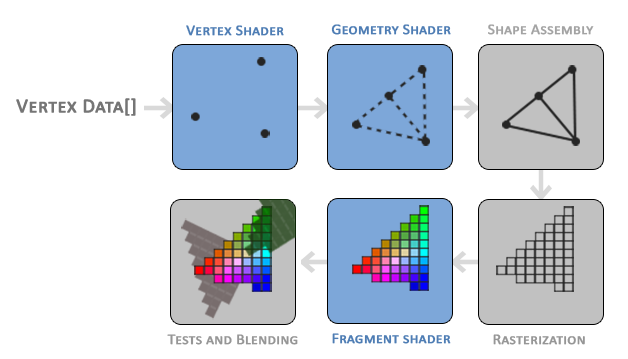
\includegraphics[width=0.8\textwidth]{pipeline.png}
    \caption{Nejdůležitěljší části vykreslovacího řetězce (modře vybarvené části jsou programovatelné)}
    \vspace{-5pt}
    {\footnotesize Zdroj: \url{https://learnopengl.com/Getting-started/Hello-Triangle}}
    \label{fig:pipeline}
\end{figure}

Ve vykreslovacím řetězci (\textit{graphics pipeline}) je vertex shader jeden z prvních. Je spuštěň pro každý bod (\textit{Vertex}), který grafické kartě pošleme a spustí na něm kód, který napíšeme. Používá se především na transformaci bodů v prostoru na obrazovku.

Po složení trojúhelníků z bodů a jejich následná rasterizace na pixely, se pro každý pixel spustí fragment shader a vykreslí výslednou barvu pixelu na obrazovku. Využívá se především na osvětlení.

\subsubsection{Deferred renderování}
V klasickém renderování se používá \texttt{forward renderování} (\textit{dopředného vykreslování}), kde pokaždě když zavoláme, aby byl objekt vykreslen, tak ho rovnou i osvětlíme, což znamená, když bude jiný objekt ten první překrývat, tak jsme ztratili čas počítáním osvětlení na pixelu, který byl následně přepsán.

Tento engine využívá techniku s názvem \texttt{deferred renderování} (\textit{odložené vykreslování}), která rozděluje vykreslování na geometry pass, do kterého vykreslíme čistá data objektů na obrazovce a následně v lighting passu všechno najednou osvětlíme. Tento postup urychluje výkon, při větším počtu světel, za cenu komplexity a různých grafických efektů, jako je průhlednost.


\subsection{Herní UI}
Jak bylo již řečeno v kapitole~\ref{sec:tech-ui}, engine používá k hernímu uživatelskému prostředí knihovnu RmlUi. Engine nijak nezapouzdřuje RmlUi. Poskytuje vývojáři \texttt{Rml::Context}, se kterým může vytvářet uživatelké prostředí v HTML a CSS. Zapouzdření knihovny by vyžadovalo značné úsilí pro identické nebo možná i horší vývojářské pohodlí používání.


\subsection{Application}
Tato třída je rozhraní, přes které uživatel komunikuje s enginem. Jak je patrné z diagramu na obrázku \ref{fig:architektura}, vlastní \texttt{Scene Manager}, \texttt{Resource Manager} a \texttt{Input Manager}. Uživatel oddědí třídu \texttt{engine::Application} a implementuje \texttt{on\_start} a \texttt{on\_update}.

\subsection{Entity a scény}
Engine spravavuje objekty, pomocí zjednodušeného návrhového vzoru ECS (\textit{Entity Component System}). ECS rozděluje funkčnost objektů na komponenty, které obsahují jenom samostatná data, následně na entity, které se skládají z komponent a naposledy systémy, které zpracují data z komponenty a provedou určitou logiku.

Jak již bylo řečeno, engine využívá zjednodušenou verzi ECS, kde komponenty jsou funkční samy o sobě. Toto řešení bylo zvoleno, kvůli příliš velké komplexitě implementování rozdělenosti komponent a funkčnosti nezjednodušené verze a zároveň minimálního užitku.

\subsubsection{Entita}
Všechny objekty v enginu jsou entity, jako je například hlavní kamera, podlaha, hráč,  budova a další objekty ve scéně.

Hlavní účel \texttt{entit} je uchovávat list komponent a umožnit vývojáři jednoduché operace s nimi, jako jsou \textit{add}, \textit{remove} a \textit{contains}. Dovoluje hierarchické vztahy typu rodič-potomek (\textit{Parent-Child}), který zajistí, že každý potomek zdědí transformaci (posun, rotace a škálování) rodiče.

\subsubsection{Komponenty}
Komponentu, kterou má každá entita je \texttt{Transform}, která uchovává pozici, rotaci a velikost entity. Engine tyto vlastnoti následně využije v počítání modelové matice.

Důležitá, ale dobrovolná komponenta je \texttt{Mesh}, která je převážně zodpovědná za to, jaký model má engine vykreslit.

Na úpravu vzhledu entity existují \texttt{Material} a \texttt{Texture} komponety.

Další důležité komponenty jsou \texttt{Camera}, \texttt{Light} a \texttt{Collidery}.

\subsubsection{Scéna}
Primární práce \texttt{scény} je evidovat a vlastnit entity, které od ní uživatel přidá. Vlastní také třídu zodpovědnou za kolize.

\subsubsection{Scene Manager}
\texttt{Scene Manager} je zodpovědný za evidenci a vlastnění scén. Poskytuje funkce k přepínání mezi scénami dle jména a načítání scény ze souboru.


\subsection{Resource Manager}
K jednoduché práci s texturama a modelama, poskytuje třída \texttt{engine::Application} \texttt{Resource Manager}, který je dovoluje jednoduše načítat a získávat. 

\subsubsection{Texture Manager}
Primární práce \texttt{Texture Manageru} je uchovávání ukazatelů na textury, uložené na grafické kartě. Obsahuje také i takzvaně nezbytné textury, bez kterých se engine nespustí. Jsou to textury hlavně na správnou funkčnost renderování a textura, která bude zobrazena, pokud se učitou texturu nepovede načíst.

\subsubsection{Mesh Manager}
\texttt{Mesh Manager} je abstrakce nad OpenGL objekty (\textit{VBO}, \textit{EBO} a \textit{VAO}), které jsou zodpovědné za nahrávání dat modelů na grafickou kartu. Umožňuje přidání modelů ze souboru, ale poté co začne hra (skončí funkce \texttt{on\_start}), aby byl model přidán na grafickou kartu, musí být Mesh Manager rekompilován, pomocí funkce \texttt{compile()}.

\subsection{Input Manager} \label{sec:input-manager}
Aby hra mohla být interaktivní, potřebuje vývojář, nějak přistupovat ke vstupu uživatele. Třída \texttt{Input Manager} je udělaná pro jednoduchý a rychlý přístup ke vstupu od klávesnice a myši.



\section{Implementace enginu}

\subsection{Inicializace a hlavní herní smyčka}

Vstupním bodem každé aplikace založené na Rainfall Enginu je funkce \texttt{engine::run}, které dáte vaši třídu, která dědí z \texttt{engine::Application}.

\begin{lstlisting}[caption={Vstupní bod aplikace}]
#include <engine/core/Engine.h>
#include "ExampleGame.h"

int main()
{
    engine::run<ExampleGame>();
    return 0;
}
\end{lstlisting}

Životní cyklus každé aplikace je rozdělen na inicializaci (\textit{start}), herní smyčku a vypnutí (\textit{shutdown}).
První věc, která nastane je inicializace, kde se vytvoří okno, RmlUi, renderovací systém a instance vaší odděděné aplikace.

\subsubsection{Herní smyčka}
Po inicializaci se spustí hlavní herní smyčka, která je zodpovědná za neustálý běh aplikace, dokud ji uživatel nebo popřípadě vývojář neukončí.

\begin{lstlisting}[caption={Herní smyčka}]
while (app.is_running() && !window.should_close())
{
    // Update
    rmlui_layer.update(*app.input_manager);
    renderer.update();
    app.update(renderer.delta_time);
    // Render
    renderer.render();
    rmlui_layer.render(window.get_width(), window.get_height());
    renderer.swap_and_poll();
}
\end{lstlisting}

Nejdříve se spustí update funkce pro renderer a aplikaci vývojáře, až pak se spustí renderování.


\subsection{Renderování}
\subsubsection{Stíny}
K vytváření stínů engine využívá techniku \texttt{Shadow mapping}. Z ortografického pohledu směrového světla (\textit{directional light}) vyrenderuje hloubkovou mapu aktuální scény do textury, kterou následně použije osvětlovací systém, aby spočítal, kam světlo vidí a kam ne. Tento způsob vytváření stínů je relativně rychlý a vypadá dostatečně dobře.

\subsubsection{Geometry pass}
V této části renderování se podle každé entity v aktuální scéně nastaví různé proměnné, dle koponent, co entita vlastní, a pak se zavolá vykreslení dané entity.

Každý vertex, který jsme poslali grafické kartě na vykreslení, musí projít vertex shaderem, kde ho převede z \textit{localního prostoru} do \textit{clip prostoru}, pomocí součinu několika matic.

\begin{equation}
    V_{clip} = M_{projection} \times M_{view} \times M_{model} \times V_{local}
\end{equation}

Výsledkem je bod, který je na správné relativní pozici vůči kameře. Tuto rovnici spočítá pro každý vertex paralelně.

Následně se data užitečná pro osvětlení každé entity vykreslí do několika textur. Například pozice modelu na každém pixelu, anebo barva (materiál nebo textura) entity na každém pixelu. Dohromady těmto texturám se říká \texttt{G-Buffer}.

\subsubsection{Lighting pass}
Po nahrání dat do G-Bufferu, je na řadě \texttt{Lighting pass}, aby spočítal, jak má být každý pixel nasvícen. Nejdříve nastaví globální proměnné, jako je pozice kamery, specifikace mlhy a hlavně nastaví data světel.

K osvětlení engine používá \texttt{physically based rendering} \cite{learnopengl} (\textit{PBR}), který se snaží imitovat světlo, aby dodržovalo zákony fyziky. Na rozdíl od mnohem jednodušší techniky Blinn-Phong, vypadá mnohlem lépe a dovoluje větší svobodu v možnostech materiálů.

Physically based rendering k renderování používá specializovanou verzi render equation (\textit{zobrazovací rovnice}) s názvem reflectance equation.

\begin{equation} \label{eq:reflectance}
L_o(p, \omega_o) = \int_{\Omega} f_r(p, \omega_i, \omega_o) L_i(p, \omega_i) (n \cdot \omega_i) \, d\omega_i
\end{equation}

\noindent kde:
\begin{itemize}
    \item[$L_o(p, \omega_o)$] je výsledné odražené záření (\textit{outgoing radiance}),
    \item[$f_r$] představuje funkci BRDF (\textit{Bidirectional Reflectance Distribution Function}),
    \item[$L_i(p, \omega_i)$] je přicházející záření ze směru $\omega_i$,
    \item[$(n \cdot \omega_i)$] je kosinusový úhel mezi normálou plochy a směrem dopadajícího světla,
    \item[$d\omega_i$] je diferenciální prostorový úhel integrace.
\end{itemize}

Logika výpočtu reflectance equation je implementována v GLSL shaderu\footnote{\href{https://github.com/Rohlicek128/rainfall_engine/blob/master/engine/src/Rendering/Shaders/GLSL/Lighting/pbr\_lighting.frag}{pbr\_lighting.frag}}.

\subsubsection{Post process pass}
Výsledek z lighting passu je vyrenderován do textury, kterou následně použije \texttt{post process pass}, k spočítání různých grafických efektů.

Jeden z těchto efektů je \texttt{HDR} (\textit{High Dynamic Range}), která umožňuje správně vykreslovat velmi silná a slabá světla v jednom obraze, bez toho aby barvy přesahovaly limit 1.0 a ukazovaly se jako bílá, což by znamenalo ztrátu informací v obraze.

Pro dosažení realistického vizuálního výstupu implementuje engine systém automatické expozice, který simuluje adaptaci lidského oka na světelné podmínky scény.

\begin{equation}
C_{out} = \left( C_{in} \cdot \frac{k}{Y_{avg} \cdot 2^t} \right)^{\frac{1}{\gamma}}
\end{equation}

\noindent kde:
\begin{itemize}
    \item[$C_{out}$] je výsledná barva v prostoru LDR (\textit{Low Dynamic Range}),
    \item[$C_{in}$] je barva v HDR prostoru (\textit{High Dynamic Range}),
    \item[Y] zastupuje průměrný jas scény (\textit{Average Luminance}),
    \item[k] je parametr \textit{Key Value} (cílový jas scény),
    \item[t] je \textit{Threshold} (posun expozice),
    \item[$\gamma$] je hodnota gama korekce (obvykle 2.2).
\end{itemize}

V posledním kroku je barva transformována z lineárního prostoru do prostoru s gama korekcí, což zajišťuje správné zobrazení na běžných monitorech.

Logika výpočtu automatické expozice a gamy je implementována v GLSL shaderu\footnote{\href{https://github.com/Rohlicek128/rainfall_engine/blob/master/engine/src/Rendering/Shaders/GLSL/Screen/screen.frag}{screen.frag}}.



\section{Tvorba obsahu v enginu}
Celý vývoj aplikace nebo hry se odehrává primárně v odděděné třídě \texttt{engine::Application}.

\begin{lstlisting}[caption={Vytvoření ukázkové aplikace}]
#include <engine/core/Application.h>

class ExampleGame : public engine::Application
{
public:
    void on_start() override;
    void on_update(const float delta_time) override;
};
\end{lstlisting}

\begin{lstlisting}[caption={Ukázka definice scény a entit v C++}]
void ExampleGame::on_start()
{
    // Konfigurace projektu - pro distribuci se project_dir necha prazdny
    current_project->project_dir = "";

    // Vytvoreni sceny a hlavni entity
    Scene* scene = scene_manager->create_scene("MainScene", true); // true, aby se scena nastavila jako current_scene
    Entity* box = scene->create_entity("PlayerModel");

    // Pridavani komponent 
    box->add_component<MeshComponent>(0); // ID modelu

    Texture* tex = resource_manager->load_texture("assets/textures/character.jpg", "jpg");
    box->add_component<TextureComponent>(tex);
    box->add_component<engine::physics::SphereCollider>();
    box->add_component<PlayerScript>(); // Vlastni herni logika

    // Vytvoreni bodoveho svetla
    Entity* light = scene->create_entity("PointLight");
    light->transform->position = glm::vec3(3.0f, 2.0f, 2.0f);
    light->add_component<LightComponent>(lights::LIGHT_TYPE::POINT, glm::vec3(1.0f, 1.0f, 0.8f));
}
\end{lstlisting}

\subsubsection{Správa cest a přenositelnost}
Důležitým architektonickým prvkem je správa proměnné \texttt{project\_dir} v objektu \texttt{current\_project}.
\begin{itemize}
\item \textbf{Vývoj v editoru:} Zde se využívá absolutní cesta (např. \texttt{C:\textbackslash{}Projects\textbackslash{}Rainfall\textbackslash{}}), aby editor přesně věděl, kam ukládat serializované YAML soubory a odkud načítat assety nezávisle na pracovním adresáři.
\item \textbf{Distribuce (Build):} Pro koncové spuštění na jiném počítači se tato hodnota nastavuje jako prázdný řetězec. Engine v tomto případě automaticky přepíná na relativní cesty, což zajišťuje, že aplikace správně nalezne složky \texttt{assets/} a \texttt{scenes/} v kořenovém adresáři spustitelného souboru.
\end{itemize}

Tento systém umožňuje plynulý přechod mezi vizuální editací v editoru a finálním nasazením aplikace bez nutnosti měnit zdrojový kód nebo strukturu souborů.



\subsection{Registrace vstupu hráče}
K registaci vstupu hráče, lze, jak již bylo zmíněno v kapitole~\ref{sec:input-manager} dosáhnout pomocí třídy \texttt{Input Manager}, která je zodpovědná za vstup klávesnice a myši.

\subsubsection{Vstup klávesnice}

\begin{lstlisting}[caption={Ukázkové získání vstupu klávesnice}]
void ExampleGame::on_update(const float delta_time)
{
    if (input_manager->get_key_up(GLFW_KEY_R))
    {
        // logika
    }
    if (input_manager->get_key_down(GLFW_KEY_S))
    {
        // logika
    }
    if (input_manager->get_key_toggle(GLFW_KEY_T))
    {
        // logika
    }
    if (input_manager->get_key_with_timeout(GLFW_KEY_U, 1000))
    {
        // logika
    }
}
\end{lstlisting}

\begin{itemize}
    \item \textbf{Get key up:} Spustí se, jen pokud je klávesa \textit{GLFW\_KEY\_R} nezmáčknutá.
    
    \item \textbf{Get key down:} Spustí se, jen pokud je klávesa \textit{GLFW\_KEY\_S} zmáčknutá.
    
    \item \textbf{Get key toggle:} Spustí se po stisknutí klávesy \textit{GLFW\_KEY\_T}, ale aby se tato část spustila znovu, musí klávesu nejdříve pustit a pak znova stisknout.

    \item \textbf{Get key with timeout:} Spustí se po stisknutí klávesy \textit{GLFW\_KEY\_U}, ale aby se tato část spustila znovu, musí počkat 1000 milisekund, než bude klávesa znovu spustitelná.
\end{itemize}

\subsubsection{Vstup myši}

\begin{lstlisting}[caption={Ukázkové získání vstupu myši}]
void ExampleGame::on_update(const float delta_time)
{
    if (input_manager->mouse->get_button_up(GLFW_MOUSE_BUTTON_1))
    {
        // logika
    }
    if (input_manager->mouse->get_button_down(GLFW_MOUSE_BUTTON_2))
    {
        // logika
    }
    if (input_manager->mouse->is_scrolling_y())
    {
        // logika
    }
}
\end{lstlisting}

\begin{itemize}
    \item \textbf{Get button up:} Spustí se, jen pokud je \textit{GLFW\_MOUSE\_BUTTON\_1} (levé tlačítko myši) nezmáčknuté.
    
    \item \textbf{Get button down:} Spustí se, jen pokud je \textit{GLFW\_MOUSE\_BUTTON\_2} (pravé tlačítko myši) zmáčknuté.
    
    \item \textbf{Is scrolling y:} Spustí se, jen když se otáčí kolečko u myši. K získání, o kolik se kolečko otočilo, použijte \textit{input\_manager->mouse->scroll\_y\_delta}.
\end{itemize}

K získání aktuální pozice myši na obrazovce v pixelech lze získat proměnné \textit{input\_manager->mouse->pos\_x} a \textit{input\_manager->mouse->pos\_y}.



\subsection{Vlastní logika entit}
Pro vytvoření vlastní logiky pro entity, je možné použít \texttt{Behaviour} komponentu k vlastnímu skiptování. Stejně jako \texttt{engine::Application}, má vlastní funkce \texttt{on\_start}, \texttt{on\_update} a \texttt{on\_shutdown}.

Pokud bychom chtěli, aby se daná entita s touto komponentou točila do kola, musíme v \texttt{on\_update} funkci použít proměnnou \textit{self}, která ukazuje na vlastnící enitu komponenty. Také si budeme ukládat i proměnnou \textit{count}, která se po každém spuštění \texttt{on\_update} zvedne o \textit{delta time}. Tuto proměnnou použijeme k plynulé rotaci entity.

\begin{lstlisting}[caption={Vytvoření ukázkového behaviour skriptu v TestScript.h}]
#include <engine/world/components/BehaviorComponent.h>

class TestScript : public BehaviorComponent
{
public:
    void on_start() override;
    void on_update(const float delta_time) override;
private:
    float count_;
};
\end{lstlisting}

\begin{lstlisting}[caption={Rotace objektu v skriptu TestScript.cpp}]
#include "TestScript.h"
#include <engine/world/Entity.h>
#include <cmath>

void TestScript::on_start()
{
    count_ = 0.0f;
}

void TestScript::on_update(const float delta_time)
{
    count_ += delta_time;
    self->transform->position.x = std::sin(count_) * 2.0f;
    self->transform->position.z = std::cos(count_) * 2.0f;
}
\end{lstlisting}

K vytvořerní komplexnější logiky, můžeme vytvořit \textit{trigger}, což je entita s kolizní komponentou, která po dotyku s ostatní entitou a také s kolizní komponentou, spustí kus kódu.

Například kdybychom chtěli posunout každou entitu, která se dotkne entity s \textit{TestScript} komponentou, tak se posune o 10 jednotek nahoru. V \textit{TestScript.h} přepíšeme funkci (\textit{function overriding}) \texttt{on\_trigger} a v \textit{TestScript.cpp} dopíšeme logiku.

\begin{lstlisting}[caption={Přidání on\_trigger v TestScript.h}]
public:
    void on_trigger(Entity& other, const engine::physics::CollisionsPoints& points) override;
\end{lstlisting}

\begin{lstlisting}[caption={Logika on\_trigger v TestScript.cpp}]
void TestScript::on_trigger(Entity& other, const engine::physics::CollisionsPoints& points)
{
    other.transform->position.y += 10.0f;
}
\end{lstlisting}




\section{Editor}

Samotný herní engine představuje sadu programátorských rozhraní (API) a systémů běžících na pozadí. Aby byl engine efektivně využitelný pro tvorbu obsahu, byl k němu vyvinut dedikovaný grafický editor. Tento editor není pevnou součástí enginu, ale funguje jako samostatná aplikace, která plně využívá jeho API. Slouží tak zároveň jako komplexní ukázka praktického použití vyvinuté knihovny. Koncepčně lze editor vnímat jako pokročilé vizuální rozhraní pro serializaci a úpravu strukturovaných datových souborů YAML.

\begin{figure}[H]
    \centering
    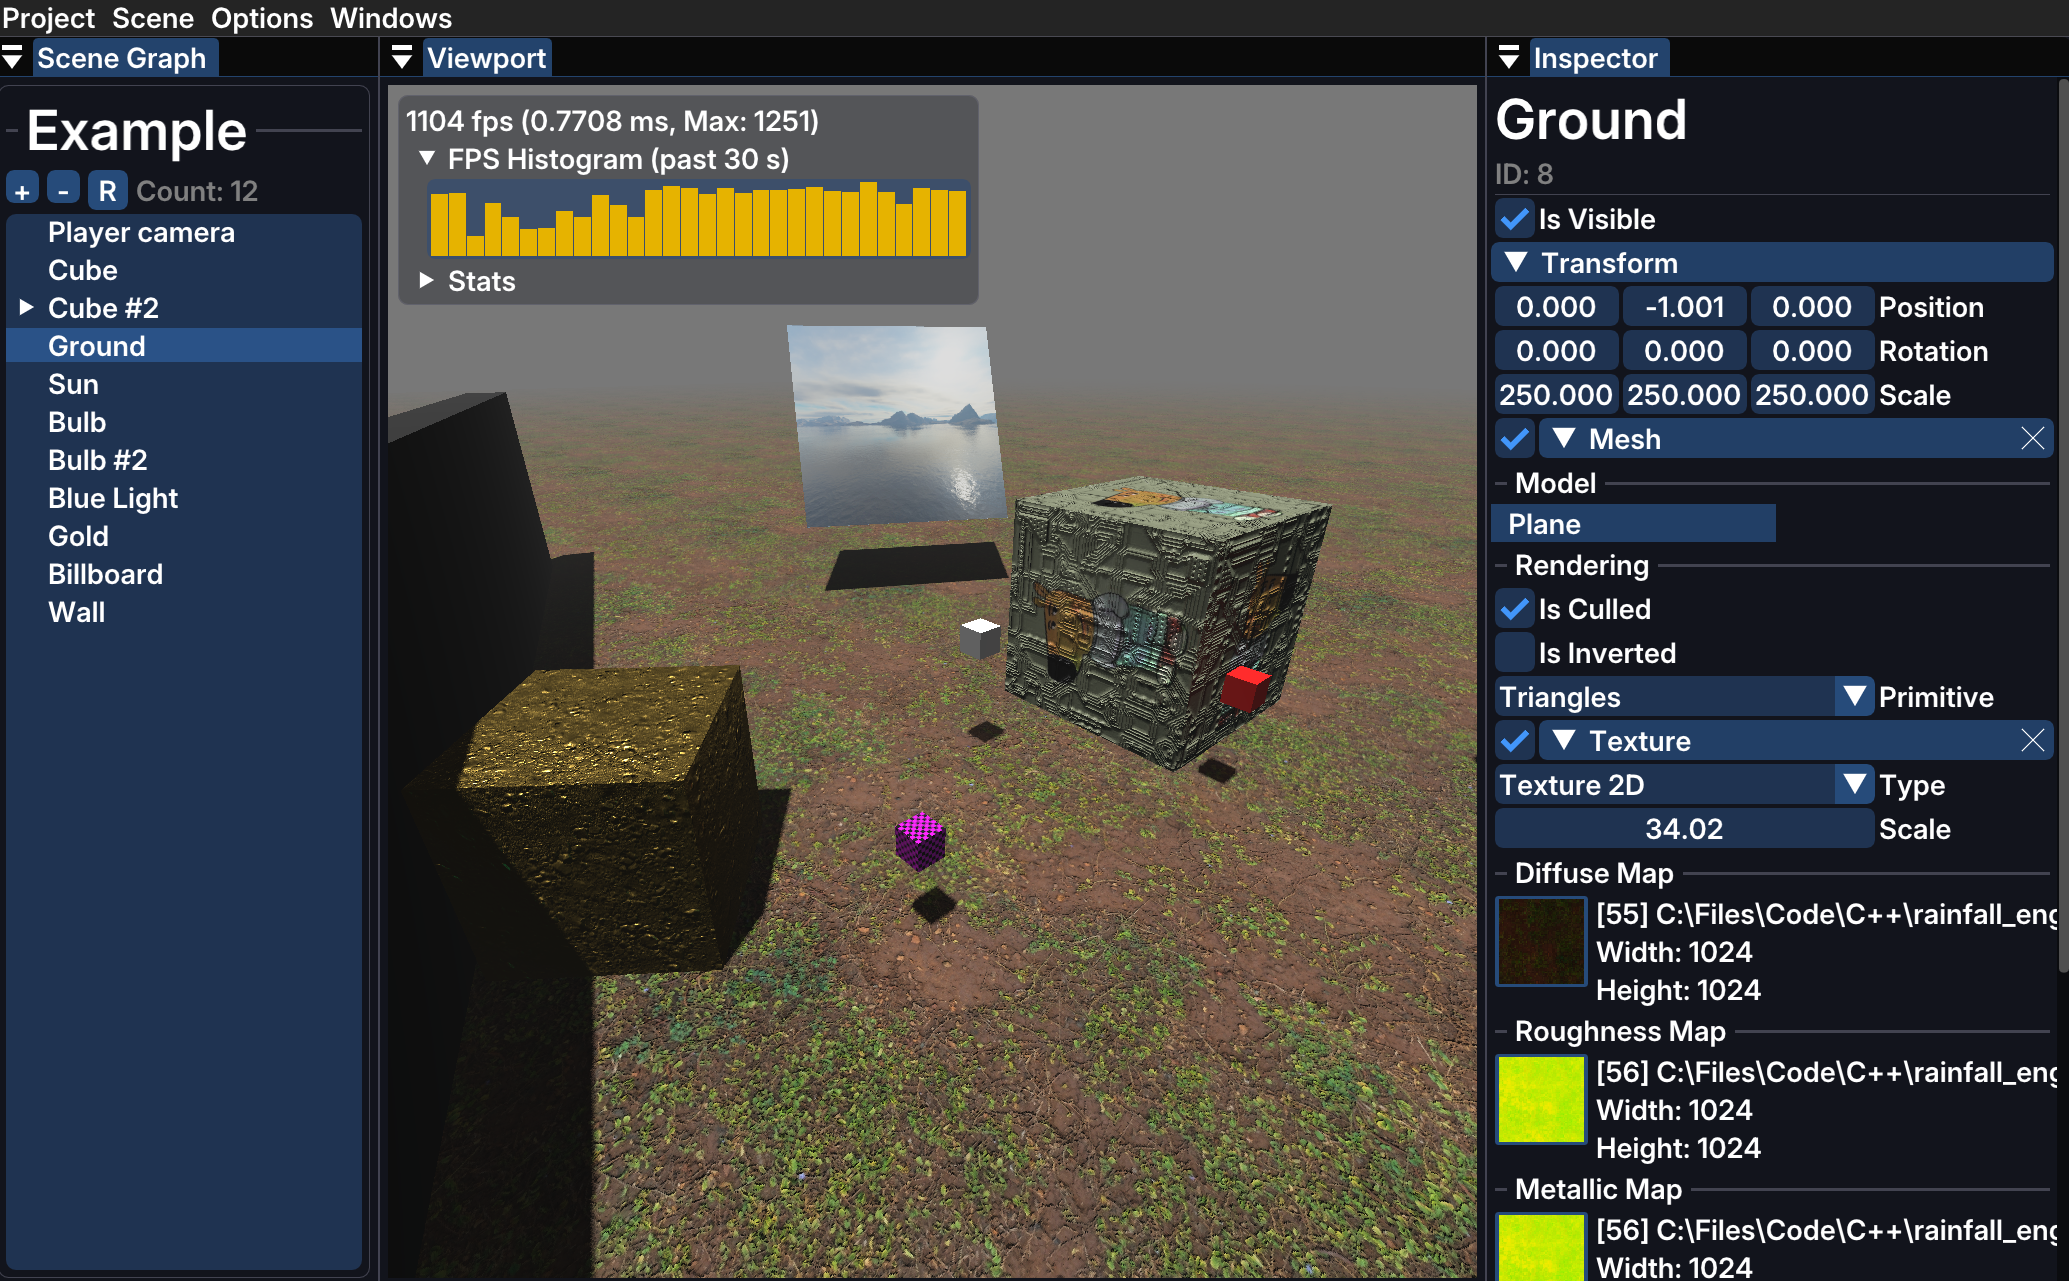
\includegraphics[width=0.9\textwidth]{editor.png}
    \caption{Rozhraní editoru a Dear ImGui UI}
    \label{fig:editor}
\end{figure}

\subsection{Integrace knihovny Dear ImGui}
Pro tvorbu uživatelského rozhraní byla zvolena populární C++ knihovna \texttt{Dear ImGui}\cite{imgui}. Jedná se o tzv. \textit{Immediate Mode GUI}, které je ideální pro vývoj nástrojů reálného času, jelikož nevyžaduje složitou správu stavů ovládacích prvků. Integrace s enginem spočívá v napojení knihovny na existující kontext okna (GLFW) a grafickou pipeline (OpenGL).

Editor plně využívá funkci \textit{Docking} (dokování oken), která uživateli umožňuje libovolně přesouvat, spojovat a organizovat jednotlivé panely (\textit{Dockspace}) podle jeho aktuálních potřeb, podobně jako to umožňují profesionální komerční nástroje.

\subsection{Nástroje editoru}
Uživatelské rozhraní je rozděleno do několika logických panelů, které poskytují kontrolu nad různými aspekty herní scény a chodu aplikace.

\subsubsection{Správa projektů a scén}
Proces ukládání a načítání je v editoru rozdělen na dvě úrovně: projekty a scény. Celkové nastavení aplikace se ukládá do souborů s příponou \texttt{.rainp} (Rainfall Project). Samotná hierarchie entit, jejich komponenty a nastavení prostředí jsou serializovány do formátu YAML a ukládány jako soubory scén s příponou \texttt{.rain}. Editor umožňuje plynulé přecházení mezi scénami a jejich modifikaci v reálném čase.

\subsubsection{Viewport a monitorování výkonu}
Hlavním vizuálním prvkem editoru je panel \textit{Viewport}. Scéna není vykreslována přímo do hlavního okna aplikace, ale do vlastního Framebuffer objektu (FBO), jehož výsledná barevná textura je následně předána ImGui k zobrazení jako obrázek. Tento přístup odděluje vykreslování hry od vykreslování uživatelského rozhraní.

Součástí editoru je také diagnostický panel pro monitorování běhu enginu. Obsahuje informace o aktuálním čase běhu aplikace (\textit{Uptime}), hodnotu \textit{Delta Time} a aktuální snímkovou frekvenci (FPS). Pro lepší vizualizaci stability výkonu je k dispozici histogram zachycující historii FPS za posledních 30 sekund.

\begin{figure}[H]
    \centering
    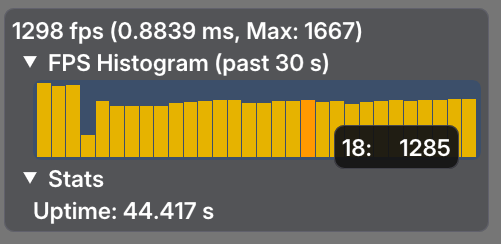
\includegraphics[width=0.5\textwidth]{editor_performance.png}
    \caption{Panel zobrazující aktuání výkon}
    \label{fig:editor-performance}
\end{figure}

\subsubsection{Graf scény}

\begin{wrapfigure}{r}{0.5\textwidth}
    \centering
    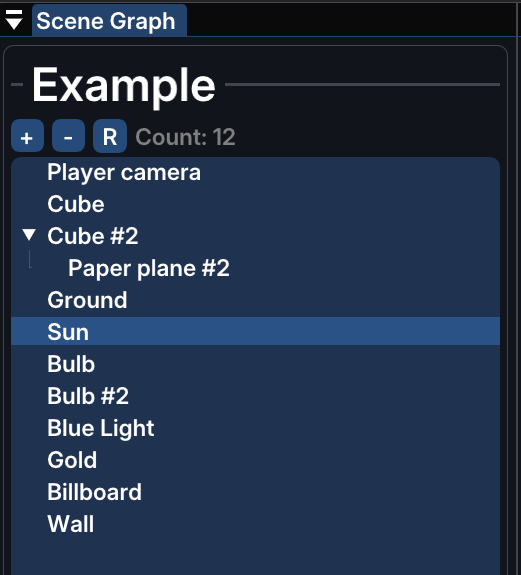
\includegraphics[width=0.45\textwidth]{editor_scene_graph.png}
    \caption{Stromový graf entit ve scéně}
    \label{fig:editor-scene-graph}
\end{wrapfigure}

Panel \textit{Scene Graph} (Hierarchie) zobrazuje strukturu aktuálně načtené scény ve formě stromového grafu. Každý herní objekt je reprezentován jako entita. Editor plně podporuje hierarchické vztahy typu rodič-potomek (\textit{Parent-Child}). Tato stromová struktura zajišťuje, že transformace (posun, rotace, změna měřítka) aplikované na rodičovskou entitu se automaticky kaskádovitě přenášejí i na všechny její potomky.




\subsubsection{Inspektor entit}
Po výběru konkrétní entity v grafu scény se její detaily zobrazí v panelu \textit{Inspector}. Tento nástroj slouží k úpravě vlastností vybrané entity. Uživatel zde může dynamicky přidávat nové komponenty (např. \textit{MeshComponent}, \textit{MaterialComponent}, \textit{LightComponent}) a upravovat jejich hodnoty. Změny parametrů v Inspektoru se díky přímému napojení na API enginu okamžitě projevují ve Viewportu.



\section{Ukázková aplikace a technologické demo}
Aby bylo možné v praxi ověřit funkčnost a stabilitu navržené architektury enginu, byl v rámci projektu vytvořen funkční herní prototyp. Tato ukázková aplikace neslouží jako finální a uzavřený herní produkt, ale funguje primárně jako technologické demo a tzv. \textit{Proof of Concept}. Jejím hlavním cílem je demonstrovat reálnou integraci jednotlivých subsystémů enginu od grafického vykreslování, přes systém entit a komponent (ECS), zpracování uživatelského vstupu, až po základní fyzikální detekci kolizí a vykreslování uživatelského rozhraní (UI).

\subsection{Herní smyčka a mechaniky}
Prototyp je koncipován jako jednoduchá 3D arénová hra o přežití. Hráč ovládá kameru z pohledu první osoby, přičemž se volně pohybuje po vyhrazené ploše pomocí klávesnice (WASD) a myši. Logika pohybu a rozhlížení je implementována prostřednictvím vlastního skriptu \texttt{CameraScript}, který zpracovává data z \texttt{InputManageru}.

Herní smyčka je dynamická a plně využívá možnosti \texttt{SceneManageru} pro instancování objektů za běhu aplikace (\textit{runtime}). V pravidelných intervalech jsou na náhodných pozicích generovány entity nepřátel. Každému nepříteli je přiřazena komponenta \texttt{EnemyScript}, která obsahuje jednoduchou umělou inteligenci zajišťující sledování pozice hráče a pohyb směrem k němu.

\subsection{Fyzika a správa paměti}
Pro obranu má hráč k dispozici možnost střelby. Každý výstřel dynamicky vytvoří novou entitu projektilu (\texttt{Bullet}). Na tomto mechanismu je demonstrována práce s fyzikálním subsystémem: jak nepřátelé, tak projektily využívají komponentu \texttt{Sphere Collider}. Fyzikální engine v každém snímku vyhodnocuje průniky těchto sférických obálek. Pokud dojde ke kolizi (událost \texttt{on\_trigger}), nepřítel změní barvu materiálu a klesne pod úroveň terénu, což simuluje jeho eliminaci.

Ukázka kódu níže demonstruje, jak je v enginu řešena reakce na fyzikální kolizi mezi nepřítelem a projektilem pomocí události \texttt{on\_trigger}:

\begin{lstlisting}[caption={Reakce na kolizi v komponentě EnemyScript}]
void EnemyScript::on_trigger(Entity& other, const engine::physics::CollisionsPoints& points)
{
    if (BulletScript* bullet = other.get_component<BulletScript>())
    {
        if (bullet->entered) return;
        bullet->entered = true;

        health -= bullet->damage;
        if (health <= 0)
        {
            if (MaterialComponent* mat = self->get_component<MaterialComponent>())
                mat->color = glm::vec4(1.0f, 0.0f, 0.0f, 1.0f);
            self->transform->position.y = -0.75f;
        }
    }
}
\end{lstlisting}


\subsection{Uživatelské rozhraní}
Prototyp také demonstruje integraci 2D uživatelského rozhraní pomocí knihovny RmlUi, ktera dovoluje na obrazovce v reálném čase aktualizovat počet zbývajících životů hráče.

\subsection{Budoucí vývoj prototypu}
Současná podoba ukázkové hry představuje základní iteraci. Díky flexibilitě architektury enginu a oddělení dat od logiky je aplikace připravena na další rozšiřování.




\section{Závěr}
Cílem této odborné práce bylo navrhnout a implementovat vlastní 3D herní engine v jazyce C++, pochopit vnitřní mechanismy komerčních systémů a vytvořit plně funkční ukázkovou aplikaci. Výsledkem je projekt Rainfall Engine, který tento cíl úspěšně naplňuje a tvoří stabilní základ pro budoucí vývoj.

\subsection{Zhodnocení výsledků}
Během vývoje se podařilo vytvořit robustní architekturu, která propojuje správu paměti, herní logiku a moderní grafické API OpenGL. Engine disponuje vlastním systémem pro správu entit a komponent, systémem pro načítání 3D modelů a textur a implementuje pokročilé grafické techniky. Zvláštní důraz byl kladen na vizuální kvalitu, čehož bylo dosaženo integrací Deferred renderingu, modelu osvětlení PBR a automatické expozice v rámci HDR post-processingu.

\subsection{Možnosti dalšího rozvoje}
Architektura enginu byla navržena tak, aby umožňovala snadnou integraci nových systémů. V nejbližší budoucnosti se vývoj zaměří na následující klíčové oblasti:

\begin{itemize}
    \item \textbf{Pokročilý fyzikální systém:} Současná implementace podporuje pouze základní detekci sférických kolizí. Dalším krokem bude vývoj nebo integrace plnohodnotného fyzikálního enginu, který umožní simulaci dynamiky tuhých těles (\textit{Rigid Body Dynamics}) a detekci kolizí pro komplexní tvary (např. přes AABB nebo konvexní trupy).
    
    \item \textbf{Rozšíření renderování stínů:} Aktuální verze enginu využívá základní variantu algoritmu Shadow mapping pro směrová světla. Pro eliminaci vizuálních artefaktů a zlepšení kvality stínů v otevřených scénách je plánována implementace techniky \textit{Cascaded Shadow Maps} (CSM), která dynamicky přizpůsobuje rozlišení stínové mapy dle vzdálenosti od kamery.
    
    \item \textbf{Dokončení PBR pipeline:} Physically based rendering bude obohaceno o \textit{Image-Based Lighting} (IBL). Pomocí environmentálních HDRI map engine získá podporu pro realistické globální osvětlení a přesné odrazy na materiálech, což vizuální kvalitu posune na úroveň moderních komerčních enginů.
\end{itemize}

Projekt Rainfall Engine mi dokázal, že i přes vysokou komplexitu moderní grafiky lze s odhodláním vyvinout vlastní funkční řešení, na kterém mohu dále stavět své profesní portfolio.


% --- Literatura ---
\newpage
\begin{thebibliography}{99}

    \bibitem{learnopengl} 
    DE VRIES, Joey. \textit{LearnOpenGL} [online]. 2014. Dostupné z: \url{https://learnopengl.com/}

    \bibitem{imgui} 
    CORNUT, Omar. \textit{Dear ImGui: Bloat-free Graphical User interface for C++} [software]. Dostupné z: \url{https://github.com/ocornut/imgui}

    \bibitem{glfw} 
    GEELNARD, Marcus a Camilla LÖWY. \textit{GLFW} [software]. Dostupné z: \url{https://www.glfw.org/}

    \bibitem{glm} 
    RICCIO, Christophe. \textit{OpenGL Mathematics (GLM)} [software]. Dostupné z: \url{https://glm.g-truc.net/}

    \bibitem{assimp} 
    GESSLER, Alexander a Kim KULLING. \textit{Open Asset Import Library (Assimp)} [software]. Dostupné z: \url{https://www.assimp.org/}

    \bibitem{yamlcpp} 
    BEDER, Jesse. \textit{yaml-cpp} [software]. Dostupné z: \url{https://github.com/jbeder/yaml-cpp}

    \bibitem{khronos} 
    KHRONOS GROUP. \textit{OpenGL Documentation} [online]. Dostupné z: \url{https://docs.gl/}

    \bibitem{rmlui} 
    MIKKE89. \textit{RmlUi: The HTML/CSS User Interface Package} [software]. Dostupné z: \url{https://mikke89.github.io/RmlUiDoc/}

\end{thebibliography}

% --- Přílohy ---
\newpage
\section*{Přílohy}
\addcontentsline{toc}{section}{Seznam příloh}

\textbf{Zdrojové kódy a spustitelná verze} \\
    Kompletní zdrojové kódy projektu, assety ukázkové hry a zkompilovaný spustitelný soubor jsou dostupné v online repozitáři na platformě GitHub: \\
    \url{https://github.com/Rohlicek128/rainfall_engine}


\end{document}
